%!TEX root = thesis.tex
\chapter{Introduction}\label{c:1}
At high temperature, an isolated collection of molecules at a low enough volume fraction is a fluid and thus is a homogeneous system on average; the probability of finding any molecule at any specific position is a constant and only depends on the density of the particles.
As this system is invariant under all possible rotations and translations, we say that the system has complete continuous translational and rotational symmetry.
If we lower the temperature, the system will eventually develop order, where the individual molecules have a preferred local arrangement.
For this example, lowering the temperature will eventually induce the system to transition from a fluid phase to a crystalline phase, characterized by an underlying periodic lattice.
This order is \emph{long-range}, such that knowing the position of one particle gives the position of every other particle in the system, regardless of the distance between the particles.
Another way of stating this is that the correlation functions describing the ordered state do not decay.
Thus, the system is now only invariant with respect to a discrete set of translations and rotations.
Here, the system breaks the continuous symmetry of the isotropic phase in order to achieve the crystalline phase.
Hence, the ordered phase has lower symmetry than the isotropic phase.

The advent of long range order as a result of the spontaneous breaking of continuous symmetry is general and is a hallmark of transitions between a multitude of different phases.
In addition, the phases do not have to be formed by collections of molecules; they can be built from a variety of constituent units, from angstrom-scale atoms to micron-scale colloidal particles or even larger building blocks.
Regardless of the nature of the constituent particles, the isotropic-to-crystalline phase transition in three dimensions (3D) breaks continuous translational and rotational symmetry in all directions.
However, a system can also transition from an isotropic phase to a phase where the continuous translational and rotational symmetry is not broken in all directions.
For example, an isotropic-to-smectic phase transition in 3D breaks continuous translation symmetry in only one direction and continuous rotational symmetry in two directions, while the isotropic-to-uniaxial nematic and isotropic-to-ferromagnetic transitions break no translational symmetries and only breaks rotational symmetry in two directions~\cite{RN175}.
Breaking continuous translational symmetry results in positional order while breaking continuous rotational symmetry results in orientational order.
\begin{figure}
  
\includegraphics{figures/C1/Ch1-Figs_SmecticNematic.png}
  \caption{Smectic and nematic order.
  (A), A smectic phase breaks translational symmetry along one direction, leading to a layer-like structure.
  For the drawn Smectic-A phase, this direction is indicated by $\bm{\nu}$.
  (B), A uniaxial nematic phase has continuous translational symmetry in all directions and continuous rotational symmetry in one direction. This direction is indicated by the director, $\mathbf{n}$.}\label{f:1-SmecticNematic}
\end{figure}

With the development of order as a result of breaking one or more continuous symmetries comes the rigidity needed to maintain that order.
For example, due to their broken symmetries, crystalline, smectic, and nematic phases cannot be made to flow as easily as the isotropic phase of the material.
However, since a nematic phase has no broken continuous translational symmetries, in contrast to smectic and crystalline phases, the nematic phase of a material will flow easier than the smectic and crystalline phases of that material.
This is because the constituent particles in a nematic only need to maintain their orientation and not their position.
In addition, systems with anisotropic order have a correspondingly anisotropic rigidity.
Consider a smectic phase with its broken translational symmetry in one direction, defined by a unit vector $\bm{\nu}$, as drawn schematically in Figure~\ref{f:1-SmecticNematic}(A).
Along $\bm{\nu}$, the material will resist flow like a crystal, but will flow easily like an isotropic fluid along directions orthogonal to $\bm{\nu}$.
Similarly, even though a uniaxial nematic has continuous translational symmetry in all directions, it still has certain rigidity as the nematic must maintain its two-fold orientational order, defined by a unit vector $\bm{n}$ [see Figure~\ref{f:1-SmecticNematic}(B)].
A nematic phase resists torques that affect the orientations of $\bm{n}$. Since a force along $\bm{n}$ imposes no torque, there is no rigidity along $\bm{n}$.
In both of these examples, the rigidity depends on the direction of the deformation, and thus is anisotropic.
This phenomenon is not limited to the rigidity; in general, properties of a phase will reflect the symmetries of the phase.
For example, ordered materials often exhibit birefringence, where the index of refraction is anisotropic.
Thus, the speed of light in a birefringent material depends on the direction and polarization of the light~\cite{RN175}.

Ordered materials can also have defects, defined generally as locations in the material where the preferred arrangement is not satisfied.
Belying the colloquial definition, defects in the order are not necessarily undesirable; in fact, they can have important consequences for the physics of the phase, and thus can be exploited to achieve specific properties.
For example, joining two crystalline domains of incompatible orientations results in defects forming a border, or grain boundary, between the two domains.
In a crystalline material, these grain boundaries affect the moduli of the material, and are even responsible for the phenomenon of ``work hardening,'' where the plastic deforming of the material increases the magnitude of the shear modulus.
This is commonly done to create durable objects from copper and other ductile metals.
The plastic deformations cause isolated defects and grain boundaries to proliferate within the material; however, as the defect density rises, so does the energy required to generate new defects and move existing defects.
This results in an increased resistance to deformation that further reflects in the increase of the shear modulus.

In addition, defects can also directly mediate phase transitions, as in the celebrated Kosterlitz-Thouless-Halperin-Nelson-Young (KTHNY) theory of melting in 2D~\cite{RN161,RN162,RN163}.
In two or fewer dimensions, a system cannot spontaneously break continuous symmetry and establish LRO.
This is known as the Mermin-Wagner theorem~\cite{RN175}.
However, in 2D, a system can still have phases with quasi-long range order (QRLO).
The QRLO and associated rigidity arise from correlations between the constituent particles in the material.
However, the correlation functions in QRLO decay as a power law in the separation distance between the particles~\cite{RN175}.
For this reason, phases with QLRO are also called \emph{algebraically-ordered}.
In this case, the increase in symmetry when an algebraically-ordered 2D crystalline phase melts to the isotropic phase is a two-step process.
First, beginning in the crystalline phase, the crystalline phase will always possess pairs of thermally excited dislocations, or translational defects.
While a single dislocation will always reduce the translational order of the crystal, a pair of dislocations can have no net effect on the order.
Raising the temperature in the crystalline phase will eventually induce the dislocation pairs to \emph{unbind}.
The free dislocations reduce the translational order of the crystalline phase, but do not affect the orientational order of the system, inducing a transition from the crystalline phase to an intermediate hexatic phase characterized by six-fold orientational order~\cite{RN61,RN203}.
We note that each dislocation is composed of a pair of disclinations, or rotational defects; isolated disclinations reduce the orientational order of the system, but a pair of disclinations \emph{bound} together to form a dislocation have no net effect on the orientational order.
Raising the temperature even further will eventually induce the disclination pairs to unbind, destroying the orientational order and transforming the hexatic phase into the isotropic phase.
This phase map for this two-step process is illustrated schematically in Figure~\ref{f:1-KTHNY}.
Furthermore, defects in soft matter have been used as tools to investigate a wide range of phenomena from knot theory~\cite{RN156,RN277} to controlled self-assembly~\cite{RN43,RN50,RN150,RN157}, to hierarchical materials~\cite{RN164,RN159,RN27}.
\begin{figure}
  \centering
  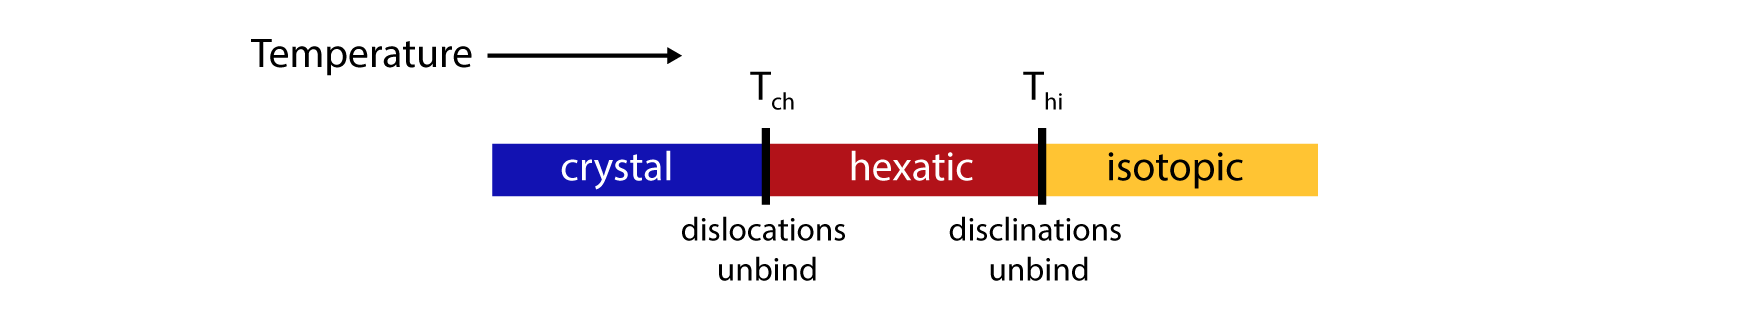
\includegraphics{figures/C1/Ch1-Figs_KTHNY.png}
  \caption{Schematic of the phase behavior for melting in 2D.
  $T_{ch}$ and $T_{hi}$ are the transition temperatures for the crystalline-hexatic transition and the hexatic-isotropic transition, respectively.
  }\label{f:1-KTHNY}
\end{figure}

Apart from both their effect on physical systems and their use as tools, defects are fascinating objects in their own right as they can both be required by the topology and interact with geometry of the space they inhabit.
Consider, for example, a dense packing of rods in a plane at zero temperature.
In order to maximize the entropy of the system, the rods need to align along the same direction, resulting in the uniaxial nematic phase~\cite{RN204}.
We characterize this preferred local alignment with a director, $\mathbf{n}$, where the inversion symmetry of the system dictates that $\mathbf{n}$ and $\mathbf{-n}$ describe the same state.
Since rotating the director by $\pi$ about an axis orthogonal to $\mathbf{n}$ does not change the state, we say that the system has 2-fold order.
Clearly, it is easy to fill space on the plane with a homogeneous director field, as shown schematically in Figure~\ref{f:1-RodsPlane}(A).
However, if we now try to pack rods on the surface of a sphere, for example along either the latitude or longitude lines of the Earth's globe [Figure~\ref{f:1-RodsPlane}(B)], we see that there are defects in the order that correspond to the singular points at the poles, where $\mathbf{n}$ is undefined.
Since one ``cannot comb a hairy ball without a cowlick,'' or singularity in the pattern of the hair, the presence of singularities is no accident --- it is a consequence of confining the nematic to the surface with the topology of a sphere~\cite{RN209,RN169}.
\begin{figure}
  \centering
  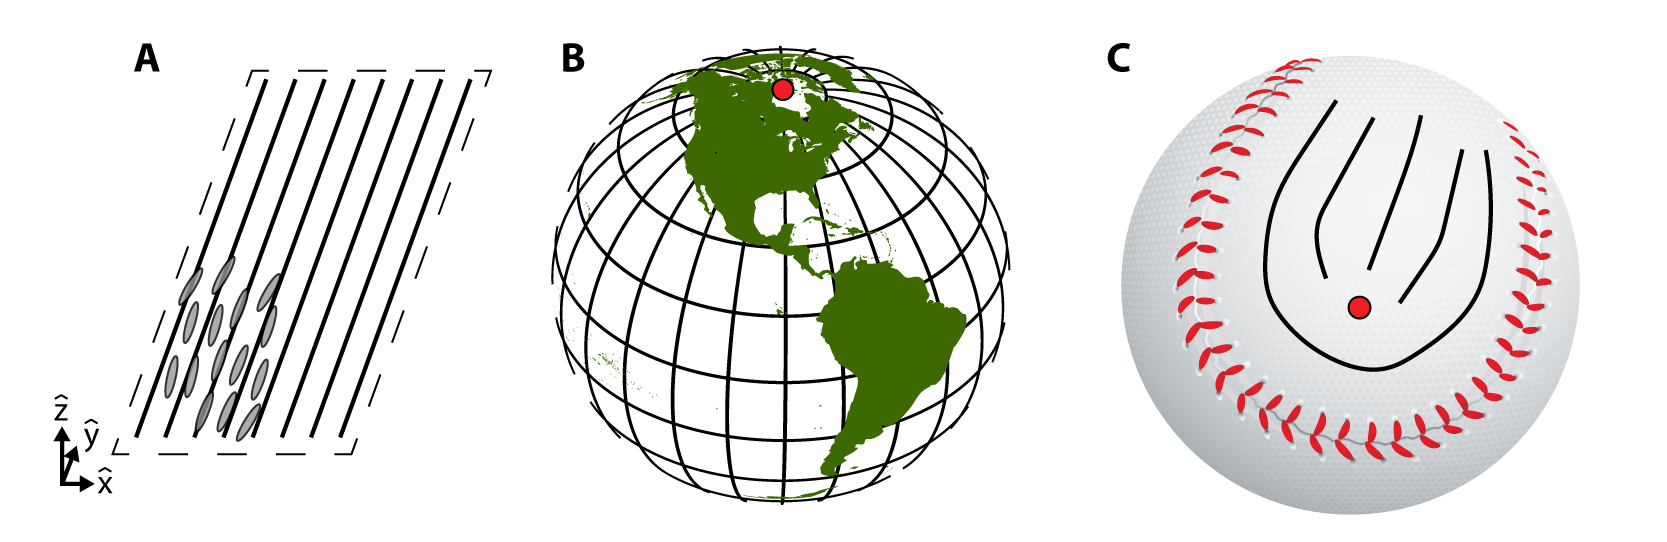
\includegraphics{figures/C1/Ch1-Figs_RodsPlane.png}
  \caption{Packing rods in two dimensions.
  (A-C), Rod-like particles preferentially align along a common axis, given by the black lines.
  (A) On a plane, the alignment can be homogeneous everywhere.
  (B,C) On a sphere, there must be singularities (${\color{red} \bullet}$) in the alignment directions, as shown for alignment directions along (B) the latitude or longitude lines on a globe and an alignment direction along (C) the stitching on a baseball.
  Note that there while only one singularity is visible in (B,C), there are 2 singularities in (B) and 4 in (C).}\label{f:1-RodsPlane}
\end{figure}

To formally relate the topology of the sphere with the presence of singularities, we need a few topological notions.
The sphere is an example of a differentiable surface that is compact, has no boundary, and is orientable.
Compact surfaces must both be bounded and contain their limit points.
Here, the term ``bounded'' means the surface has some finite size and is distinct from whether or not the surface has a boundary.
The boundary of a surface is defined as the set of points that can be approached from both the interior and the exterior of the surface.
Finally, orientable surfaces have a consistently defined normal vector everywhere.
For example, 2D Euclidean space, denoted as $\mathbb{R}^2$, is a surface but it is not bounded and thus it is not compact.
Given $\mathbf{r} \in \mathbb{R}^2$, the 2D open unit disc $|\mathbf{r}| < d$ is not compact since it does not contain the circle with radius $d$.
However, the 2D unit disc $|\mathbf{r}| \leq d$ satisfies both conditions and thus is compact.
In addition, we see that $|\mathbf{r}| \leq d$ has a boundary $\partial \mathbf{r}$ at $|\mathbf{r}| = d$, as $\partial \mathbf{r}$ can be approached by points in both the interior and the exterior of the disc.
We call surfaces that are compact and without a boundary \emph{closed surfaces}.
Finally, all of these examples are also orientable; it is trivial to define a consistent surface normal everywhere.
\begin{figure}
  \centering
  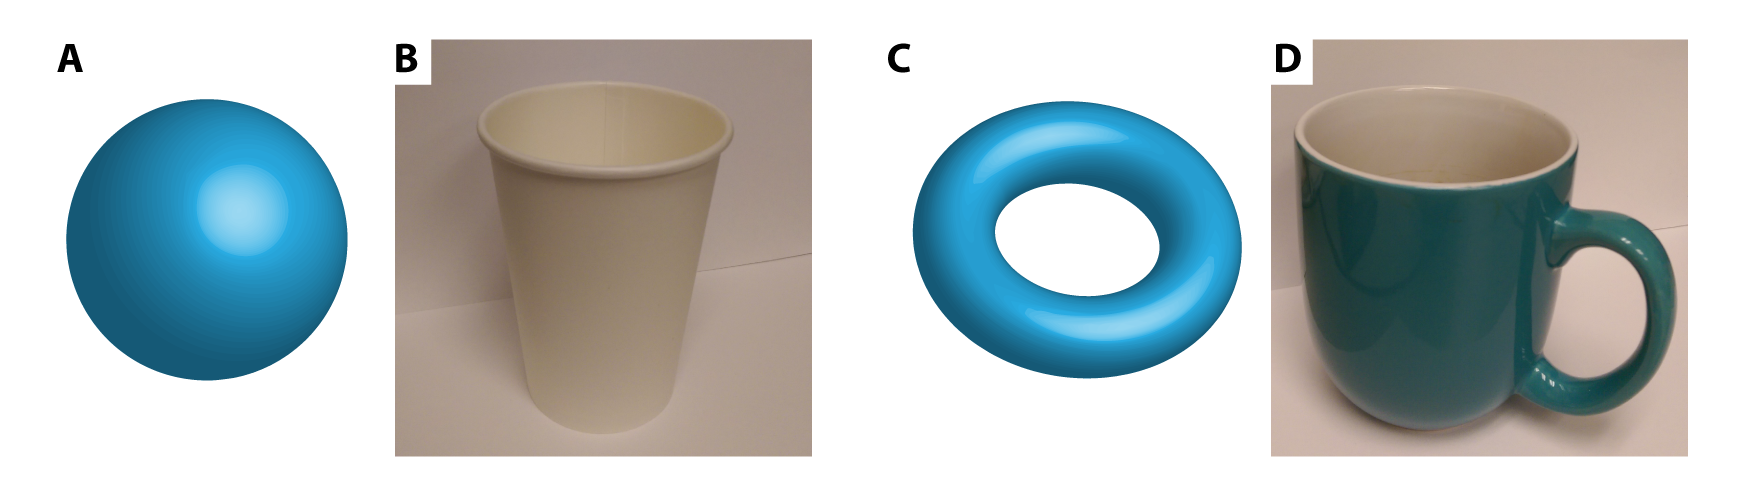
\includegraphics{figures/C1/Ch1-Figs_ChiObjects.png}
  \caption{Closed surfaces with the same Euler characteristic are homeomorphic. (A,B) Closed surfaces with no handle like a (A) sphere and (B) the surface of a cup can be continuously deformed into each other.
  (C,D) Closed surfaces with a single handle like a (C) torus and (D) the surface of a coffee mug can be continuously deformed into each other.
  However, the surfaces in (A,B) cannot be continuously deformed in the surfaces in (C,D) as the process of adding a handle breaks the surface.}\label{f:1-ChiObjects}
\end{figure}

One can characterize the topological properties of a surface via its Euler characteristic, $\chi$, which one can calculate using the Gauss-Bonnet theorem.
For a closed surface, the theorem states that~\cite{RN23}
\begin{equation}
  \chi = 2(1-g),\label{e:1-GB1}
\end{equation}
where $g$ is the genus, or number of handles, of the surface.
The Euler characteristic is a topological invariant --- continuously deforming a surface, i.e.\ under a homeomorphism, does not change its Euler characteristic.
A homeomorphism is a continuous function with a continuous inverse that maps between topological spaces while preserving topological properties.
For example, a sphere has no handles, thus $g = 0$ and $\chi=2$.
Since a homeomorphism preserves the topological properties, any surface with $g=0$ is topologically equivalent, or homeomorphic, to the sphere, and therefore also has $\chi=2$.
For example, a sphere [see Figure~\ref{f:1-ChiObjects}(A)] is homeomorphic to the surface of the kind of cup pictured in Figure~\ref{f:1-ChiObjects}(B), as neither has a handle.
Similarly, the torus and the surface of the coffee mug pictured in Figure~\ref{f:1-ChiObjects}(C,D), respectively, are also homeomorphic to each other.
However, the sphere [Figure~\ref{f:1-ChiObjects}(A)] and the torus [Figure~\ref{f:1-ChiObjects}(C)] are not homeomorphic, as one cannot add a handle to the sphere by simply bending and stretching the surface.
A handle can only be added by tearing or breaking a surface.

With these definitions, we can extend the statement, one ``cannot comb a hairy ball without a cowlick'' to, ``one cannot comb a hairy surface with $\chi=2$ without a singularity in the hair.''
In an orientation field like a director field, singularities are called ``disclinations.''
It is useful to characterize a disclination by how much the director rotates as one progresses along a closed contour encircling the disclination.
For a contour $\partial A$ and the angle $\phi(\mathbf{r})$ parameterizing the director field, with $\mathbf{r}$ being the position vector of a point on the surface, we can calculate~\cite{RN23,RN153,RN203}
\begin{equation}
  s \equiv \frac{1}{2 \pi}\oint_{\partial A} \textrm{d}\mathbf{r} \cdot \nabla\phi(\mathbf{r}) = \frac{1}{2\pi} \oint_{\partial A} \textrm{d} \phi,\label{eq:1-topCharge}
\end{equation}
where $\textrm{d}\phi$ is an exact differential.
However, since $\phi$ is not a single-valued scalar field, $\phi$ is not conservative, and $s$ is not path independent~\cite{scalarfield}.
If we map $\phi$ on $\partial A$ onto points on $\mathbb{S}^1$, the unit circle, we see that $s$ is the number of times the director field wraps the unit circle.
Since we cannot eliminate the enclosed disclination with continuous deformations of the director, disclinations are topological and $s$ is known as the winding number, or ``topological charge.''
Regardless of aligning rods along the latitudes or the longitudes on the Earth's globe, the director along a contour encircling either pole rotates by $2 \pi$, as depicted in Figure~\ref{f:1-TopCharge}(A).
Thus, both the north and the south poles have charge $s = +1$, bringing the total charge on the surface to $+2$.
The formal statement connecting a vector or director field on a closed surface with the topology of the surface is the Poincar\'e-Hopf theorem~\cite{RN23}:
\begin{equation}
  \sum\limits_{i = 1}^{N} s_i = \chi,\label{e:1-PH}
\end{equation}
where $N$ is the number of disclinations, each of topological charge $s_i$.

For nematic order, $s \in n/2$, where $n \in \mathbb{Z}$, the integers; however, for polar order, $s = n$.
For example, the defect structure in Figure~\ref{f:1-TopCharge}(B) has $s = +1/2$ and can exist for nematic order, since $\mathbf{n}$ and $\mathbf{-n}$ describe the same state.
Attempting to construct such a disclination for polar order, as illustrated by following the vectors as they go from blue to cyan along the red contour in Figure~\ref{f:1-TopCharge}(C), we see that cyan vector at the end of the path points opposite to the blue vector at the beginning of the path.
Note also that the Poincar\'e-Hopf Theorem only requires the net charge on the surface to be equal to $\chi$; we can construct a director or a vector field on a closed surface with any combination of defects so long as the total topological charge is equal to $\chi$.
\begin{figure}
  \centering
  
\includegraphics{figures/C1/Ch1-Figs_TopCharge.png}
  \caption{Topological charge of disclinations.
  (A), The director rotates by $2\pi$ along the contour enclosing the singularity (${\color{red} \bullet}$), giving $s = +1$ for both disclinations.
  (B) The director rotates by $\pi$ along the contour enclosing the singularity (${\color{red} \bullet}$), giving $s = +1/2$.
  (C) Attempting to construct an $s = +1/2$ disclination for a vector field results in a discontinuity in the vector field along the contour.
  This is seen by following the red contour as the vectors go from blue to cyan.}\label{f:1-TopCharge}
\end{figure}

In thermal equilibrium, physical ordered systems constrained to a closed surface must minimize their free energy while complying with the constraint imposed by the Poincar\'e-Hopf theorem.
For an orientationally ordered phase where the particles prefer to align parallel to each other, we can write the free energy as the cost of distorting the material from the homogeneously aligned state.
In the continuum limit, this distortion free energy is a functional of the orientation field,
\begin{equation}
  F_d = \frac{1}{2} k_F \int \textrm{d}^2r \, |\nabla \phi(\mathbf{r})|^2,\label{e:2-XY}
\end{equation}
where $k_F$ is the elastic constant governing the cost of distortion.
If we have polar order described by a vector field, then Eq.~\ref{e:2-XY} with $\phi$ and $\phi + 2\pi$ identified is a continuum description of the classical 2D X-Y model governing spins on a fixed lattice~\cite{RN175}; for nematic order, Eq.~\ref{e:2-XY} with $\phi$ and $\phi + \pi$ identified is the 2D Frank-Oseen free energy~\cite{RN61} in the 1-constant approximation~\cite{RN33}.

Nematics on a sphere were predicted~\cite{RN42,RN104,RN43} to minimize the free energy not with two $s=+1$ defects [Figure~\ref{f:1-RodsPlane}(B)] but with four $s=+1/2$ defects arranged on the vertices of a tetrahedron [Figure~\ref{f:1-RodsPlane}(C)].
Prior work in the Fern\'andez-Nieves group addressed this situation experimentally, using glass-based microfluidic devices to fabricate double emulsions~\cite{RN272}, with a shell of nematic liquid crystal (NLC) between an inner water droplet and an outer water continuous phase~\cite{RN105,RN45}.
By decreasing the osmotic pressure in the outer continuous phase of the nematic shells, swelling of the inner droplet was induced.
This swelling decreased the thickness of the NLC shell to create an experimental realization of a 2D nematic on the surface of a sphere~\cite{RN45}.
In this thin-shell limit, the four $s = +1/2$ defects arranged on the vertices of a tetrahedron was observed; see Figure~\ref{f:1-Shells}(A,B).
\begin{figure}
  \centering
  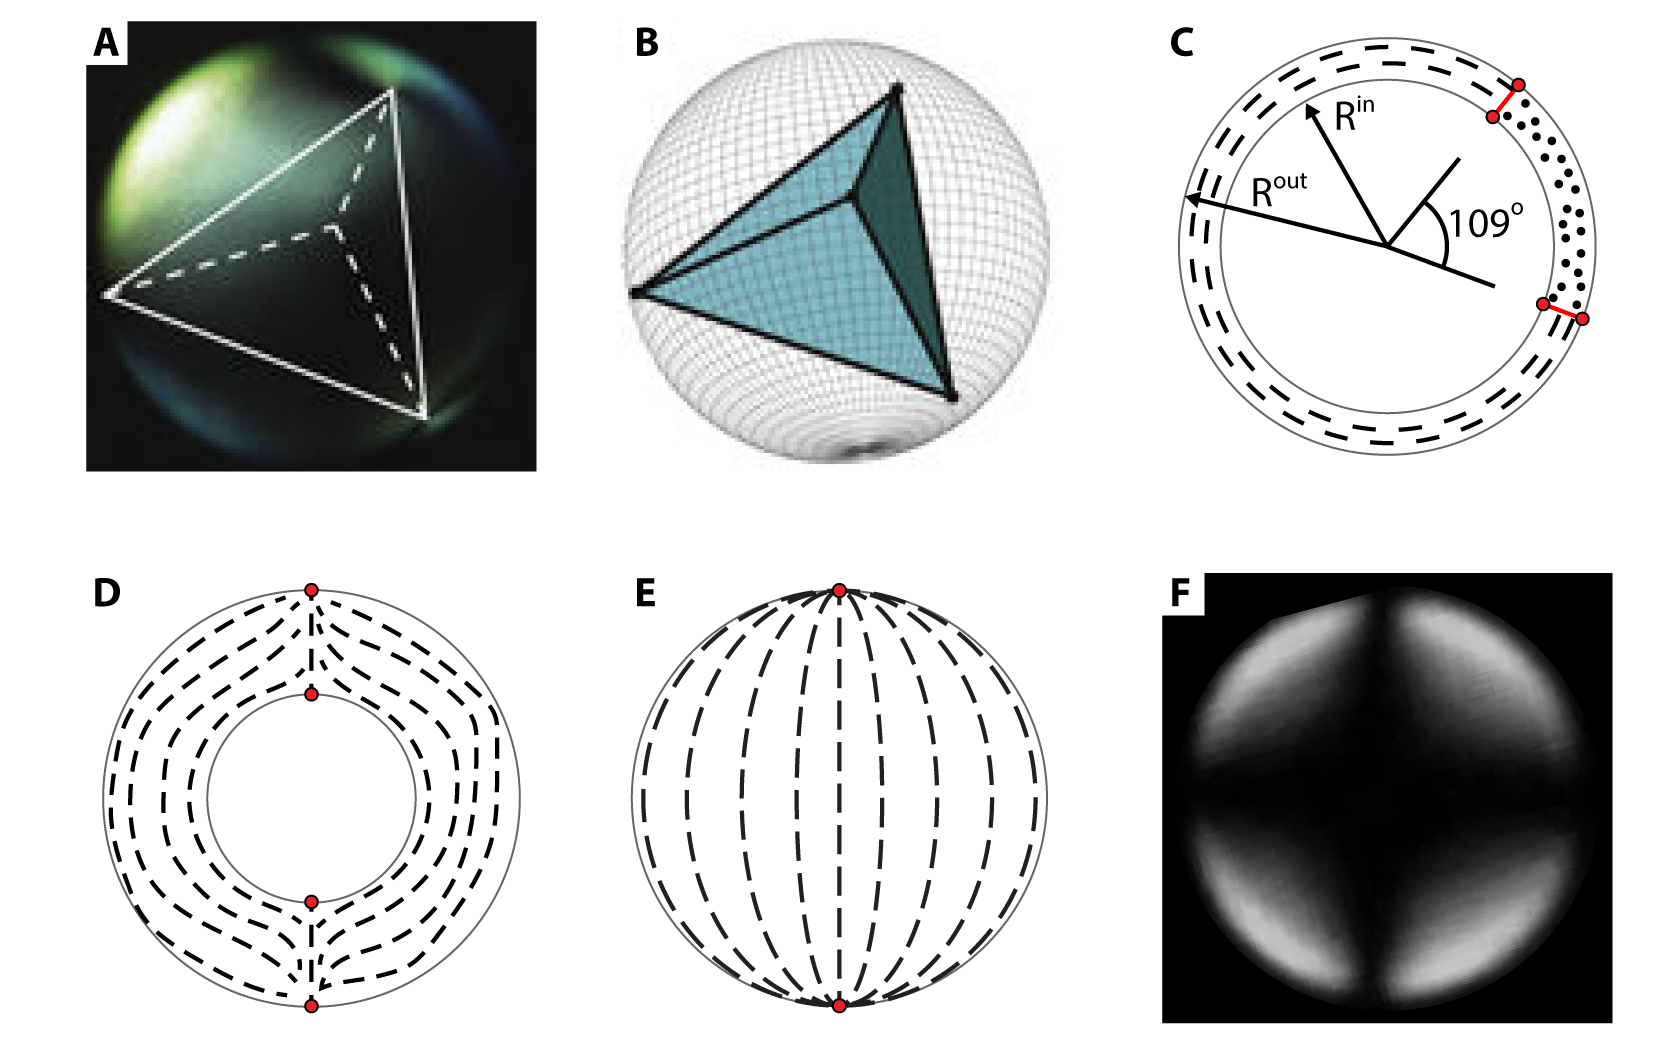
\includegraphics{figures/C1/Ch1-Figs_Shells.png}
  \caption{Shells of nematic liquid crystal.
  (A-C) Thin shells of NLC have four $s = +1/2$ defects, with an experimental crossed-polar image in (A), the tetrahedron highlighted in (B), and a cross-section schematically showing the director configuration in (C).
  The cross-section is of a great circle containing two $s = +1/2$ defects (${\color{red} \bullet}$) on both the inner and outer surface of the shell, with a red singular line connecting corresponding disclinations.
  The disclinations occupy the vertices of a tetrahedron and thus are separated by $109^{\circ}$ in the cross-section.
  (D) Cross-section of the director configuration in a thick shell. Here, the two $s = +1$ disclinations (${\color{red} \bullet}$) on each surface are no longer connected by a singular line.
  (E,F) As $R^{in}\rightarrow 0$, the thick shell becomes a bipolar droplet, with a cross-section of the director field in (E) and a corresponding crossed-polar image in (F).
  Images/Schematics in (A,B) reproduced from Ref.~\cite{RN105} with permission from Macmillan Publishers Ltd: \href{https://www.nature.com/nphys/}{Nature Physics}, copyright 2011.}\label{f:1-Shells}
\end{figure}

However, this tetrahedral arrangement of $s = +1/2$ defects only exists in thin enough shells, as characterized by the relative shell thickness $h' = (R^{out}-R^{in})/R^{out}$, with $R^{in}$ and $R^{out}$ being the inner and outer radius of the nematic shell, as defined schematically in Figure~\ref{f:1-Shells}(C).
As $h'$ is increased, the shell also becomes inhomogeneous due to density differences between the inner droplet and the NLC shell.
This thickness heterogeneity drives defects to the thinnest portion of the shell; this means that the $s = +1/2$ defects are no longer arranged in a tetrahedron.
In addition, as $h'$ is increased, the shell can no longer be considered 2D.

The situation is now 3D, and there are two spherical interfaces where the topological charge on the interface is constrained by the Poincar\'e-Hopf theorem, with a bulk region between the two surfaces filled with NLC.
Each $s = +1/2$ defect on the outer surface is then connected to a corresponding $s = +1/2$ disclination on the inner surface via a singular line that threads through the bulk.
This is depicted schematically in Figure~\ref{f:1-Shells}(C) for a great circle containing two $s = +1/2$ disclinations on each surface.
As $h'$ is increased, so does the energetic cost of each singular line.
Eventually, as $h'\gtrsim 1/2$, the energetic cost of the singular lines threading through the bulk is too great, and pairs of $s = +1/2$ disclinations each transition to a single $s = +1$ surface disclination~\cite{RN105}, known as a boojum~\cite{RN273}.

Unlike the $s = +1/2$ defects, the corresponding boojums on the inner and outer surface are not connected by a singular line; instead, the director in the shell region ``escapes into the third dimension,'' and acquires a component along the radius of the droplet, removing all the singularities in the bulk region.
The increased energetic cost of a single boojum as compared to two $s = +1/2$ defects is compensated by the energetic decrease of removing the singular regions in the bulk of the shell.
This is depicted schematically for the special case of a homogeneous shell, in Figure~\ref{f:1-Shells}(D).
For a heterogeneous thickness, the boojums migrate towards the thinnest portion of the shell.
In addition, the shells are not restricted to either four $s = +1/2$ disclinations or two $s = +1$ boojums; there are also hybrid shells with two $s = +1/2$ disclinations and a single boojum~\cite{RN105}.
For $h' = 1$, there is no inner water droplet and we have a single droplet of NLC within a continuous water phase, with the boojums on opposite poles.
This director arrangement is the classic bipolar configuration, with the director field and associated crossed polar image shown in Figure~\ref{f:1-Shells}(E,F), respectively.

This example with the shells shows that even if Eq.~\ref{e:2-XY} favors a homogeneous orientation field, corresponding to the zero elastic free energy configuration, sometimes distortions are unavoidable due to the topological constraints imposed by the surface.
However, ordered materials are also sensitive to the local geometry.
For example, consider, once more, rods packed on a plane with a homogeneous director field, as shown schematically in Figure~\ref{f:1-ParallelTransport}(A).
If we change the geometry and introduce a hemispherical ``bump'' in the plane, as illustrated in Figure~\ref{f:1-ParallelTransport}(B), evenly spaced director lines on the plane do not maintain their spacing on the bump.
Thus, we no longer have a homogeneous director everywhere on the surface.
This inability to maintain the preferred local order due to the geometry of the surface is called \emph{geometrical frustration}.
Geometrical frustration is also commonly seen in magnetic systems.
For example, it is impossible to have a triangular lattice with antiferromagnetic order everywhere; the topology of the lattice frustrates the local antiferromagnetic order, as illustrated schematically in Figure~\ref{f:1-ParallelTransport}(D).
\begin{figure}
  \centering
  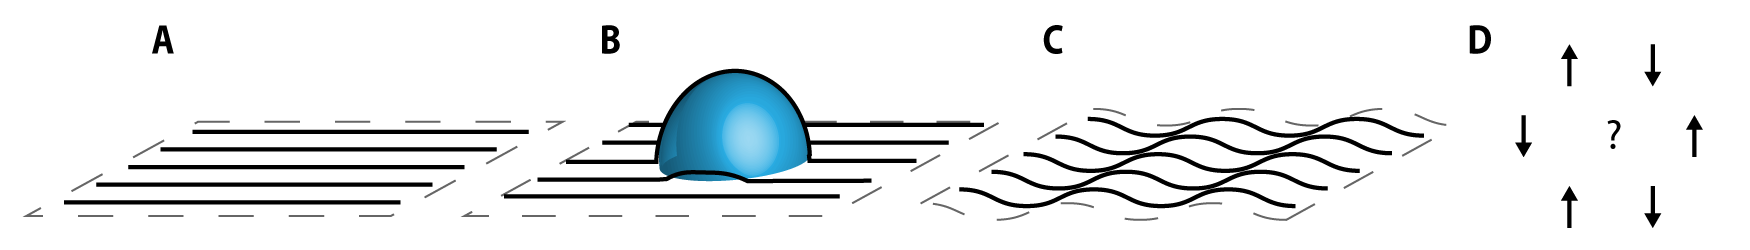
\includegraphics{figures/C1/Ch1-Figs_ParallelTransport.png}
  \caption{Geometrical frustration in nematics and in magnetism.
  (A), A flat plane can support a homogeneous director field, indicated by the black lines.
  (B), Adding a hemisphere to the plane disrupts the homogeneous state, the Gaussian curvature of the hemisphere makes a distortion-free state impossible.
  (C), Modulating the surface with a sine wave adds mean curvature but not Gaussian curvature to the surface; the homogeneous state on the surface is still possible.
  (D), Geometrical frustration in magnetism. Perfect antiferromagnetic order cannot exist on a triangular lattice.}\label{f:1-ParallelTransport}
\end{figure}

An important aspect of the local geometry of a surface is its curvature; consider a curve constrained to lie in $\mathbb{R}^2$, $\mathbf{r}(s)$, with $s$ being the arclength parameter.
Such an example of a planar curve is drawn schematically in Figure~\ref{f:1-Curvature}(A).
The unit tangent to the curve at $s$ is given by $\mathbf{T}(s) = \textrm{d} \mathbf{r}(s)/\textrm{d}s = \mathbf{r}'(s)$, and the local curvature $\kappa(s)$ by $\mathbf{k}(s)\kappa(s) = \mathbf{T}'(s) = \mathbf{r}''(s) $, with $\mathbf{k}(s)$ the unit normal vector to the curve [see Figure~\ref{f:1-Curvature}(A)] and $\kappa(s) = 1/R(s)$, where $R(s)$ is the radius of the osculating circle, or circle that best approximates $\mathbf{r}(s)$ at $s$.
This radius is commonly known as the ``radius of curvature'' at $s$.
The sign of the curvature relates to the direction $\mathbf{k}$ rotates as $s$ increases: if $\mathbf{k}$ rotates towards $\mathbf{T}$ [blue circle, see Figure~\ref{f:1-Curvature}(A)], $\kappa < 0$, while if $\mathbf{k}$ rotates away from $\mathbf{T}$ [red circle, Figure~\ref{f:1-Curvature}(A)], $\kappa > 0$.

Now consider a 2D orientable surface given by $\mathbf{R}(u^1,u^2) \in \mathbb{R}^3$, with $(u^1,u^2) \in U \subset \mathbb{R}^2$ local coordinates on the surface, and with $U$ a local coordinate patch.
We define a normal section at a point $\mathbf{r} \in U$ on the surface as the planar curve resulting from the intersection between the surface and a plane containing $\mathbf{k}(\mathbf{r})$.
Since the orientation of the plane is not unique, there are infinitely many planes that can contain $\mathbf{k}(\mathbf{r})$, and therefore infinitely many normal sections at a given point $\mathbf{r}$.
The curvature of a given normal section at $\mathbf{r}$ is called the normal curvature.
A normal section, the plane containing $\mathbf{k}$, and the osculating circle whose $R$ determines the normal curvature $\kappa(s)$, are drawn schematically in Figure~\ref{f:1-Curvature}(B) for an example surface.
Among all possible normal curvatures at $\mathbf{r}$, there is always a maximum and minimum normal curvature, with the planes containing the associated normal sections orthogonal to each other~\cite{RN35}.
These two curvatures are the \textit{principal} curvatures at $\mathbf{r}$, $\kappa_1 (\mathbf{r})$ and $\kappa_2(\mathbf{r})$, and their associated tangent vectors at $\mathbf{r}$ are the principal directions; these directions and curvatures are drawn schematically for an example surface in Figure~\ref{f:1-Curvature}(C).
From $\kappa_1$ and $\kappa_2$, we define two important quantities: the Gaussian curvature $K  \equiv \kappa_1 \kappa_2$ and the mean curvature $H \equiv  (\kappa_1+\kappa_2)/2$.

We now see that adding the hemispherical bump to the plane, which has $K = H = 0$ everywhere, changes the geometry by adding both non-zero mean and Gaussian curvatures.
However, it is the Gaussian curvature and not the mean curvature that is responsible for geometrical frustration.
We see this by considering the modulation of the flat plane with a sine wave in one direction, as shown in Figure~\ref{f:1-ParallelTransport}(C).
In this case, $K=0$ everywhere while $H$ changes throughout the surface.
Despite the fact that $H \neq 0$ everywhere, we can still maintain a homogeneous director field, in contrast to our example surface with $K \neq 0$ at the bump [Figure~\ref{f:1-ParallelTransport}(B)].
This is a reflection of the fact that Gaussian curvature is a property of the surface alone, that is, it is an \textit{intrinsic} curvature.
We can determine the Gaussian curvature of a surface without knowing anything about the space the surface is embedded in.
In contrast, determining the mean, or \textit{extrinsic}, curvature of a surface requires knowledge of the space the surface is embedded in.

Revisiting the Euler characteristic, we can rewrite the Gauss-Bonnet theorem for a differentiable closed surface as
\begin{equation}
  \chi = \frac{1}{2 \pi} \int \, K \textrm{d}^2r = 2(1-g)\label{e:1-GB2}.
\end{equation}
It is evident from Eq.~\ref{e:1-GB2} that the Gaussian curvature provides the connection between the local geometry and the topology of a closed surface.
This is a very important fact.
Even though $K$ is a property of the local \textit{geometry}, integrating $K$ over a closed surface yields a \textit{topological} invariant.
\begin{figure}
  \centering
  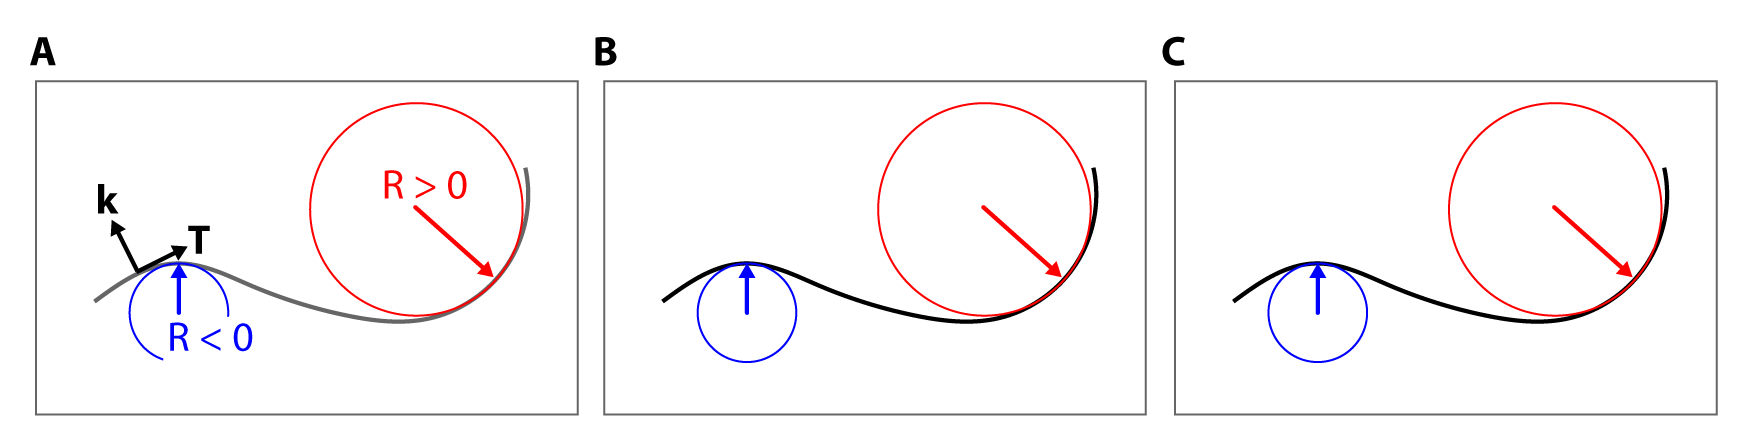
\includegraphics{figures/C1/Ch1-Figs_Curvature.png}
  \caption{Planar and surface curvature.
  (A), A planar curve with unit tangent vector $\mathbf{T}$ and unit normal vector $\mathbf{k}$. The osculating circles and associated radii of curvature are given for two points on the curve; the negative curvature is in blue and the positive curvature in red.
  (B), A normal section of a saddle-surface at a point corresponds to a planar curve, with the curve drawn in dark gray and the plane containing the curve indicated in transparent gray.
  The osculating circle and radius of curvature at the point of interest are drawn in blue.
  (C), The principal curvatures $\kappa_1$ and $\kappa_2$ at the point of interest on the surface from (B) are the maximum and minimum normal curvatures and are always in orthogonal directions. Here these directions are highlighted with the red and blue contours on the surface.}\label{f:1-Curvature}
\end{figure}

The connection between $K$ and the geometrical frustration is explicitly stated through the coupling of $K$ to the free energy of an orientationally ordered phase confined to a surface.
Considering the topological charge density
\begin{equation}
  \rho(\mathbf{r}) \equiv 2 \pi \sum\limits_i s_{i} \; \delta(\mathbf{r} - \mathbf{r}_{i}),\label{e:1-ChargeDens}
\end{equation}
due to disclinations indexed by $i$ and possessing charge $s_{i}$ and position $\mathbf{r}_{i}$, where $\delta(\mathbf{r} - \mathbf{r}_{i})$ is the Dirac delta function, we can express Eq~\ref{e:2-XY} as~\cite{RN42,RN175,RN17}
\begin{equation}
  F_d = -\frac{1}{2} k_f \int \textrm{d}^2 r \, \textrm{d}^2 r' \, G_L(\mathbf{r},\mathbf{r}') [\rho(\mathbf{r})-K(\mathbf{r})] [\rho(\mathbf{r}')-K(\mathbf{r}')],\label{e:1-TopTheoryofDefects}
\end{equation}
where $G_L$ is the Green's function of the Laplace-Beltrami operator, the standard Laplacian operator generalized to curved space~\cite{RN17}.
If we write $G_L(\mathbf{r},\mathbf{r}') = (1/2\pi) \ln |\mathbf{r} - \mathbf{r}'|$, the free-space Green's function in 2D, and make the variable change $K(\mathbf{r}) = -\Omega(\mathbf{r})$, Eq.~\ref{e:1-TopTheoryofDefects} becomes,
\begin{equation}
  F_d = -\frac{1}{4 \pi} k_f \int \textrm{d}^2 r \, \textrm{d}^2 r' \, \ln |\mathbf{r} - \mathbf{r}'| [\rho(\mathbf{r})+\Omega(\mathbf{r})] [\rho(\mathbf{r}')+\Omega(\mathbf{r}')],
\end{equation}
the Coulomb energy in 2D for a charge distribution $\rho(\mathbf{r})$ in a background of charge density $\Omega(\mathbf{r})$.
From this analogy, it is clear that topological defects couple to the Gaussian curvature of the underlying surface; in particular, defects are attracted to regions of like-signed Gaussian curvature~\cite{RN17}.

To investigate the role of curvature on ordered materials, we need to consider a space with varying Gaussian curvature and, ideally, a space including Gaussian curvatures of differing signs.
While there have been new discoveries as a result of examining defect structures on spheres~\cite{RN106,RN26,RN110,RN76,RN101,RN165}, including prior work with spherical nematic shells~\cite{RN45,RN105}, the Gaussian curvature, and therefore the background topological charge density, is constant in these cases.
As a result, the impact of curvature only enters through the sphere radius.
This is borne out in both the size-dependent onset of grain-boundary scars in colloidal crystals on the surface of emulsion drops~\cite{RN26,RN110}, and in the fact that the positions of the four $s = +1/2$ defects in nematic shells are entirely determined by the defect-defect interactions, with the underlying geometry playing no role~\cite{RN45}.

The simplest closed surface having regions of both $K>0$ and $K<0$ is the torus [Figure~\ref{f:1-ChiObjects}(C)], which has $g = 1$ and thus $\chi = 0$.
In addition, we see that not only does a torus have sphere-like, positive Gaussian curvature on its outer region and saddle-like, negative Gaussian curvature on its inner region, but according to Eq~\ref{e:1-GB2}, the integrated Gaussian curvature over an entire torus must vanish.
Similarly, by Eq.~\ref{e:1-PH}, an orientationally ordered material on the surface of a torus must have no net topological charge, and thus can support a defect-free configuration.

Prior work investigating nematic order inside a torus used toroidal droplets made from a NLC, with the nematic director constrained to lie parallel to the interface between the toroidal droplet and the outer continuous medium~\cite{RN24,RN47}.
The varying curvature of the torus yielded a double-twisted ground state with no defects~\cite{RN24}, as drawn for both a right-handed and a left-handed structure in Figure~\ref{f:1-Torus}(A,B), respectively.
Theoretically, the amount of twist in the ground state can be controlled by the aspect ratio, or slenderness of the torus $\xi = R_0/a$, with $R_0$ the radius of the central circle of the torus and $a$ the tube radius of the torus, as defined in the top view schematic in Figure~\ref{f:1-Torus}(C).
Our results revealed that the double-twist is directly related to a director distortion called saddle-splay, which favors the director in the plane of the surface aligning along the smallest principal curvature~\cite{RN24,RN59}.
In addition, as seen by the possibility of having either a right-handed or a left-handed twist, this double-twisted state manifests itself through a spontaneous reflection symmetry breaking, where the form of the free energy resembles that of the Landau theory of magnetism.
This analogy is exact for a linear twist in the cylindrical limit, where $\xi \rightarrow \infty$~\cite{RN293}.
These results clearly illustrate how confinement within surfaces of non-constant $K$ can affect the ground state of a system, even in the absence of defects.
\begin{figure}
  \centering
  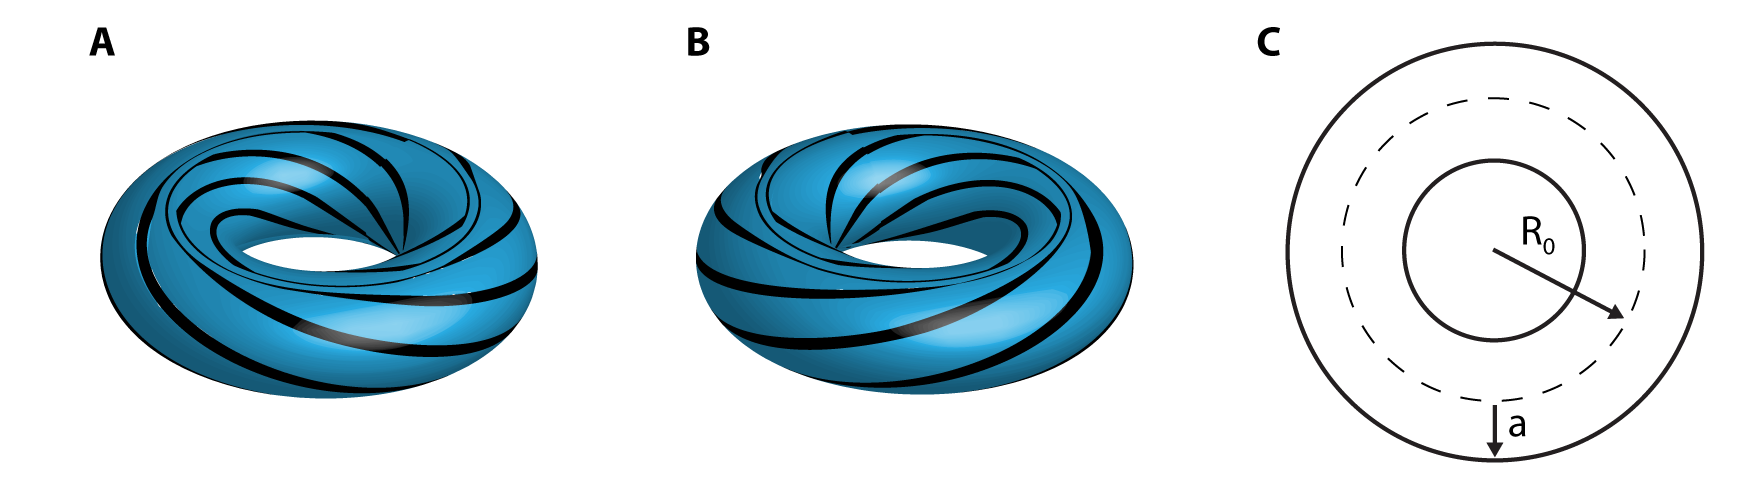
\includegraphics{figures/C1/Ch1-Figs_Torus.png}
  \caption{Doubly-twisted tori.
  (A,B), Schematics showing a (A) right-handed and (B) left-handed double-twist.
  (C), Schematic defining the central ring radius $R_0$ and tube radius $a$ in a torus.}\label{f:1-Torus}
\end{figure}

There are, however, 3D nematic fields with defects in their bulk.
For example, consider a nematic inside a volume with the director at the surface of the volume perpendicular to the surface.
We call this homeotropic anchoring.
If the volume is a sphere, we then see that irrespective of how we arrange the director in the bulk, there must be an irreducible singularity.
Bulk singularities that are points are known as hedgehogs and are characterized by their hedgehog charge,
\begin{equation}
  q = \frac{1}{4 \pi} \int_{\mathbb{S}^2} \textrm{d}\theta \: \textrm{d}\phi \: \mathbf{n} \cdot \left [ \partial_{\theta} \mathbf{n} \times \partial_{\phi} \mathbf{n} \right ],\label{e:1-HedgehogCharge}
\end{equation}
where the integral is taken over a topologically spherical surface enclosing the defect, and $\theta$ and $\phi$ are, respectively, the polar and azimuthal angles on that surface~\cite{RN153}.
In this case, instead of counting the number of times the director wraps around $\mathbb{S}^1$, as we did for the topological charge, we consider the orientation of $\mathbf{n}$ on the spherical surface enclosing the defect mapped to $\mathbb{S}^2$, the unit sphere.
The director serves as the map,
\begin{align}
  \mathbf{n} : \mathbb{S}^2 &\rightarrow \mathbb{S}^2 \nonumber \\
               (\theta, \phi) &\mapsto \mathbf{k}(\theta,\phi), \nonumber
\end{align}
where $\mathbf{k}$ is a vector normal to the ``surface'' defined by the the director.
The integrand in Eq.~\ref{e:1-HedgehogCharge} is the determinant of the Jacobian matrix of the map; it counts the area swept out on the target sphere by $\mathbf{n}$ on the surface enclosing the defect.
Thus, the hedgehog charge is then the number of times the orientations of $\mathbf{n}$ cover $\mathbb{S}^2$~\cite{RN153}.
Therefore, confining a NLC to a volume that is topologically spherical with homeotropic boundary conditions must yield a total ``hedgehog charge'' $|q|=1$.

In this Thesis, we investigate the role of geometry in the interplay between order and confinement.
In Chapter 2, we begin with an introduction to the theory of nematic liquid crystals.
Then, in Chapter 3, we consider nematic order on the surface of a torus.
This is different from previous studies where the NLC filled the torus~\cite{RN24,RN274,RN44}.
Due to the difficulty of creating a thin, stable, toroidal shell of a NLC, we use a polymeric nematic that self-assembles at the interface between two immiscible liquids.
Importantly, with this system we can generate stable toroidal droplets as in our previous work, and investigate 2D nematic order on a toroidal surface.
In addition, the nematic is active, meaning that the individual constituent particles have their own source of internal energy.
The activity then drives the nematic out of equilibrium at the individual particle level, generally causing the generation of pairs of $s = \pm 1/2$ defects that are constantly in motion and constantly being created and annihilated.
Even though we have an inherently nonequilibrium material, we find that predictions built upon Eq.~\ref{e:1-TopTheoryofDefects} hold and that adding activity to order qualitatively resembles bringing an equilibrium system to the high temperature limit.
However, there are significant differences with equilibrium nematics, which we will highlight.

In Chapter 4, we consider a NLC confined to toroidal droplets with homeotropic anchoring.
With the director constrained to lie perpendicular to the surface, the saddle-splay distortion does not affect the free energy minimization.
However, we still find a twisted ground-state configuration, where the amount of twist depends on $\xi$, eventually disappearing as $\xi \rightarrow \infty$.
Experiments with NLC confined to straight and bent cylindrical capillaries under homeotropic boundary conditions reveal that the twist is a response to the additional curvature induced when deforming a cylinder of homeotropic nematic into a torus.
This is new; prior experiments in cylinders found a twisted ground state only when NLC that favor twist distortions were used.
In our case, the confining geometry induces twist even in NLC that do not preferentially favor twist distortions.

In Chapter 5, we return to a spherical topology, confining NLC to a capillary bridge with homeotropic anchoring to study the influence of confinement shape on defect type.
We generate waist-shaped and barrel-shaped bridges and find that waist-shaped bridges contain hyperbolic defects with negative hedgehog charge while barrel-shaped bridges contain radial defects with positive hedgehog charge.
In addition, we find that the ratio of the bridge height to its width determines whether the singularity is a ring defect or a hedgehog.

In Chapter 6, we summarize, conclude, and present results that open the door to future work that builds on this Thesis.
